The problem of \emph{parsing} text into relevant and specified structures and performing operations on them is one of the most fundamental problems in computer science. 
Many problems in computer use can be broken down to fit such a description.

Prime example for a physicist could be the source-code of this very document, written in \LaTeX, or the instruction in the Python-script that runs the simulations. 
Both are just text, that needs to be parsed, dissected into relevant parts, re-arranged in computer-memory and connected to instructions, that make the computer form the simulation or output document.

The problem is known as first \emph{lexing} (sectioning a continuous stream of \emph{characters}/\emph{symbols} into \emph{words} with a different possible properties).
Directly after this, one needs to \emph{parse} these words to detect structures and extra information, derived from this structure (like e.g. parentheses, that change the order of operations for some operators).

The fine-details of such a process can vary wildly from application to application. 
General overview and guidelines to how such a process may be designed, could be found in sources like \cite{compilersDragonBook}.

In general, any mathematical equation can be represented as a \emph{tree} of operators.
So in this application, a stream of characters needs to be lexed into mathematical operators, numbers and supplementary symbols.
Then these symbols need to be parsed into an operator tree, following the \emph{grammar} on mathematical notation and extra (convenience) features one desires/requires. 

Why the act of converting a character stream into a tree is not quite straight forward and why the tree is the correct data-structure to represent terms, can be seen on the simple example presented in \autoref{fig:infix-postfix-praefix}

\begin{figure}[htbp]
    \centering
            \centering

\begin{tabular}{l|cc|ccccccc} 
    \toprule
    a&b&c\\
    \midrule 
    a&b&c\\
    a&b&c\\
    \bottomrule
\end{tabular}
\vspace{0.5cm}

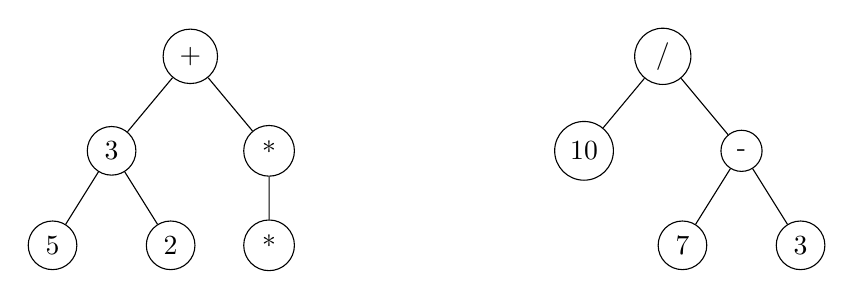
\begin{tikzpicture}[level distance=1.2cm,
    level 1/.style={sibling distance=2cm},
    level 2/.style={sibling distance=1.5cm}]

    \node[circle,draw] {+}
        child { 
            node[circle,draw] {3} 
            child { node[circle,draw] {5} }
            child { node[circle,draw] {2} }
        }
        child { 
            node[circle,draw] {*}
            child { 
                node[circle,draw] {*}
            }
        };

    \begin{scope}[xshift=6cm]

        \node[circle,draw] {/}
            child { 
                node[circle,draw] {10} 
            }
            child { 
                node[circle,draw] {-}
                child { node[circle,draw] {7} }
                child { node[circle,draw] {3} }
            };

    \end{scope}
\end{tikzpicture}
    \vspace{0.8cm}
    \caption{Display of two operator-trees for two different mathematical expressions. 
    The nodes in the branches of the tree hold operators, while the leaves generally hold numbers. These examples could be expanded through the introduction of variables and many more features that are implemented in Math-Manipulator. But the general structure is the same as in the implemented program.}
    \label{fig:infix-postfix-praefix}
\end{figure}

It shows that depending on the notation (here examples shown for \emph{postfix}, \emph{prefix} and \emph{infix}), unique operator-tree can have multiple valid notations. 
General math notation uses mainly infix notation, however some operators like faculty are postfix and functions are a type of infix.
This coupled with special/convenience features, like multiplications that could be omitted or not and many more, make this an interesting and challenging problem to tackle.